\documentclass[tikz]{standalone}

\usetikzlibrary{calc,decorations.markings}
\usepackage{amsfonts,amsmath,amsthm,amssymb,mathtools,stmaryrd,mathrsfs}

\begin{document}
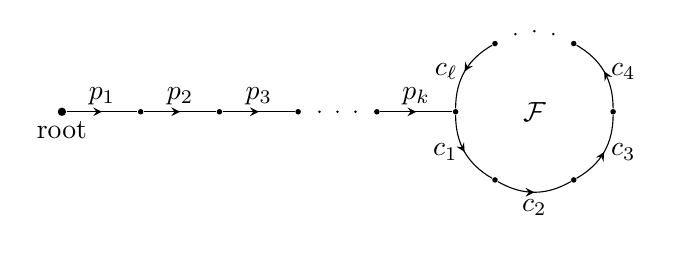
\begin{tikzpicture}[>=stealth,
	]

	\tikzset{middle arrow/.style={
				postaction=decorate,
				decoration={
						markings,
						mark=at position 0.5 with {\arrow{>}}}}
	}
	\tikzset{dotted pattern/.style={
				postaction=decorate,
				decoration={
						markings,
						mark=
						between positions 0.25 and 0.75 step 0.25
						with
							{
								\fill[radius=0.5pt,black] (0,0) circle;
							}
					}
			}
	}

	\node[circle,fill=black,inner sep=0pt,minimum size=3pt] (root) at (0,0){} node[below]{root};

	\node [circle,fill=black,inner sep=0pt,minimum size=2pt] (n1) at (1,0) {};
	\draw[middle arrow] (root) --node[above=-1pt]{$p_1$} (n1);

	\node [circle,fill=black,inner sep=0pt,minimum size=2pt] (n2) at (2,0) {};
	\draw[middle arrow] (n1) --node[above=-1pt]{$p_2$} (n2);

	\node [circle,fill=black,inner sep=0pt,minimum size=2pt] (n3) at (3,0) {};
	\draw[middle arrow] (n2) --node[above=-1pt]{$p_3$} (n3);

	\node [circle,fill=black,inner sep=0pt,minimum size=2pt] (n4) at (4,0) {};
	\draw[draw=none,dotted pattern] (n3) -- (n4);

	\node [circle,fill=black,inner sep=0pt,minimum size=2pt] (n5) at (5,0) {};
	\draw[middle arrow] (n4) --node[above=-1pt]{$p_k$} (n5);

	\node [circle,fill=black,inner sep=0pt,minimum size=2pt] (m1) at ($(5,0) + (1,0) + ({cos(180 + 60)},{sin(180 + 60)})$) {};
	\draw[middle arrow] (n5) to [bend right] node[left=-1pt]{$c_1$} (m1);

	\node [circle,fill=black,inner sep=0pt,minimum size=2pt] (m2) at ($(5,0) + (1,0) + ({cos(180 + 60*2)},{sin(180 + 60*2)})$) {};
	\draw[middle arrow] (m1) to [bend right] node[below=-1pt]{$c_2$} (m2);

	\node [circle,fill=black,inner sep=0pt,minimum size=2pt] (m3) at ($(5,0) + (1,0) + ({cos(180 + 60*3)},{sin(180 + 60*3)})$) {};
	\draw[middle arrow] (m2) to [bend right] node[right=-1pt]{$c_3$} (m3);

	\node [circle,fill=black,inner sep=0pt,minimum size=2pt] (m4) at ($(5,0) + (1,0) + ({cos(180 + 60*4)},{sin(180 + 60*4)})$) {};
	\draw[middle arrow] (m3) to [bend right] node[right=-1pt]{$c_4$} (m4);

	\node [circle,fill=black,inner sep=0pt,minimum size=2pt] (m5) at ($(5,0) + (1,0) + ({cos(180 + 60*5)},{sin(180 + 60*5)})$) {};
	\draw [draw=none,dotted pattern] (m4) to [bend right] (m5);

	\draw[middle arrow] (m5) to [bend right] node[left=-1pt]{$c_\ell$} (n5);


  \node[] (text) at (6,0) {$\mathcal F$};

\end{tikzpicture}
\end{document}
